% =========================
% L22.tex
% =========================

\chapter{L22 -- Funzioni di Lyapunov, stima della RAS e primi esempi}
\label{chap:L22}

\section{Definizione di funzione di Lyapunov}

Nella lezione precedente abbiamo visto il teorema diretto di Lyapunov: se esiste una funzione
\[
V:\mathbb{R}^n \to \mathbb{R}
\]
positiva definita e la sua derivata lungo le traiettorie è non positiva, allora l'origine è stabile; se tale derivata è strettamente negativa fuori dall'origine, allora l'origine è asintoticamente stabile.

Da qui nasce la definizione seguente.

\medskip

\noindent
\textbf{Definizione.}
Consideriamo un sistema autonomo con equilibrio nell'origine:
\[
\dot x = f(x), \qquad f(0)=0,
\]
oppure, nel caso discreto,
\[
x^{+}=f(x), \qquad f(0)=0.
\]
Una funzione \(V\) si dice \textbf{funzione di Lyapunov} per il sistema se:
\begin{itemize}
    \item \(V(0)=0\);
    \item \(V(x)>0\) per ogni \(x\neq 0\) in un intorno dell'origine, cioè \(V\) è positiva definita;
    \item la derivata lungo le traiettorie soddisfa
    \[
    L_fV(x)\le 0
    \]
    nel caso continuo, oppure
    \[
    \Delta V(x)=V(f(x))-V(x)\le 0
    \]
    nel caso discreto.
\end{itemize}

Se addirittura vale
\[
L_fV(x)<0 \quad \forall x\neq 0
\]
oppure
\[
\Delta V(x)<0 \quad \forall x\neq 0,
\]
si parla spesso di \textbf{funzione di Lyapunov stretta}.

\medskip

\noindent
In altre parole:
\begin{itemize}
    \item \(V\) deve comportarsi come una specie di energia;
    \item lungo i movimenti del sistema questa energia non deve crescere;
    \item se decresce strettamente, il sistema tende effettivamente all'equilibrio.
\end{itemize}

\section{Primo esempio: \(\dot x=-x^3\)}

Consideriamo il sistema scalare
\[
\dot x=-x^3, \qquad x\in\mathbb{R}.
\]

\subsection{Equilibrio e intuizione qualitativa}

Gli equilibri si trovano imponendo \(\dot x=0\):
\[
-x^3=0 \quad \Longrightarrow \quad x=0.
\]
Quindi l'unico equilibrio è l'origine.

Dal segno del campo vettoriale:
\[
x>0 \Longrightarrow \dot x<0,
\qquad
x<0 \Longrightarrow \dot x>0.
\]
Dunque il moto punta sempre verso l'origine.

\begin{figure}[h!]
\centering
\begin{tikzpicture}[scale=1.0]
    \draw[->] (-4,0) -- (4,0) node[right] {$x$};
    \fill (0,0) circle (1.5pt);
    \node[below] at (0,0) {$0$};

    \draw[-{Latex[length=3mm]},thick] (3,0.35) -- (2,0.35);
    \draw[-{Latex[length=3mm]},thick] (1.8,0.35) -- (0.8,0.35);

    \draw[-{Latex[length=3mm]},thick] (-3,0.35) -- (-2,0.35);
    \draw[-{Latex[length=3mm]},thick] (-1.8,0.35) -- (-0.8,0.35);
\end{tikzpicture}
\caption{Campo di direzione sulla retta per \(\dot x=-x^3\): tutti i moti puntano verso l'origine.}
\end{figure}

Questa sola osservazione suggerisce che l'origine sia asintoticamente stabile.

\subsection{Metodo indiretto}

Linearizziamo in \(x=0\). Poiché
\[
f(x)=-x^3,
\]
si ha
\[
A=\frac{df}{dx}=-3x^2.
\]
Valutando nell'equilibrio:
\[
A_0 = -3\cdot 0^2 = 0.
\]
Quindi il sistema linearizzato è
\[
\dot z = 0.
\]

Il metodo indiretto di Lyapunov qui non conclude nulla, perché l'unico autovalore è
\[
\lambda=0,
\]
cioè ha parte reale nulla.

\subsection{Metodo diretto di Lyapunov}

Proviamo con la funzione naturale
\[
V(x)=x^2.
\]
Essa è positiva definita. La derivata lungo le traiettorie è
\[
L_fV(x)=\frac{dV}{dx}f(x)=2x(-x^3)=-2x^4.
\]
Per ogni \(x\neq 0\),
\[
-2x^4<0.
\]
Quindi \(L_fV\) è negativa definita.

Per il teorema diretto di Lyapunov, l'origine è \textbf{asintoticamente stabile}.  
Questo conferma l'intuizione qualitativa iniziale e mostra bene una situazione tipica: il metodo indiretto è inconcludente, mentre il metodo diretto funziona perfettamente.

\section{Secondo esempio: \(\dot x=x^3\)}

Consideriamo ora
\[
\dot x=x^3.
\]

L'equilibrio è ancora
\[
x=0.
\]
Ma stavolta il campo vettoriale cambia completamente significato:
\[
x>0 \Longrightarrow \dot x>0,
\qquad
x<0 \Longrightarrow \dot x<0.
\]
Quindi il moto si allontana dall'origine da entrambi i lati.

\begin{figure}[h!]
\centering
\begin{tikzpicture}[scale=1.0]
    \draw[->] (-4,0) -- (4,0) node[right] {$x$};
    \fill (0,0) circle (1.5pt);
    \node[below] at (0,0) {$0$};

    \draw[-{Latex[length=3mm]},thick] (2,0.35) -- (3,0.35);
    \draw[-{Latex[length=3mm]},thick] (0.8,0.35) -- (1.8,0.35);

    \draw[-{Latex[length=3mm]},thick] (-2,0.35) -- (-3,0.35);
    \draw[-{Latex[length=3mm]},thick] (-0.8,0.35) -- (-1.8,0.35);
\end{tikzpicture}
\caption{Campo di direzione sulla retta per \(\dot x=x^3\): i moti si allontanano dall'origine.}
\end{figure}

Se scegliamo ancora
\[
V(x)=x^2,
\]
otteniamo
\[
L_fV(x)=2x(x^3)=2x^4.
\]
Per ogni \(x\neq 0\),
\[
2x^4>0.
\]
Dunque, per il criterio di Lyapunov, l'origine è \textbf{instabile}.

Questo esempio è il duale del precedente: stessa funzione \(V\), ma segno opposto di \(L_fV\), e quindi conclusione opposta.

\section{Terzo esempio piano: una dinamica non lineare con rotazione}

Consideriamo il sistema
\begin{equation}
\label{eq:L22-sistema-rotazione}
\begin{cases}
\dot x_1 = x_1\bigl(x_1^2+x_2^2-1\bigr)-x_2,\\[4pt]
\dot x_2 = x_1+x_2\bigl(x_1^2+x_2^2-1\bigr).
\end{cases}
\end{equation}

Questo sistema è interessante perché combina:
\begin{itemize}
    \item una parte radiale, governata da \(x_1^2+x_2^2-1\),
    \item una parte rotazionale, data dai termini \(-x_2\) e \(x_1\).
\end{itemize}

\subsection{Calcolo degli equilibri}

Poniamo \(\dot x_1=\dot x_2=0\):
\[
\begin{cases}
x_1(r^2-1)-x_2=0,\\
x_1+x_2(r^2-1)=0,
\end{cases}
\qquad r^2=x_1^2+x_2^2.
\]
Dalla prima ricaviamo
\[
x_2=x_1(r^2-1).
\]
Sostituendo nella seconda:
\[
x_1 + x_1(r^2-1)^2 = 0,
\]
cioè
\[
x_1\Bigl(1+(r^2-1)^2\Bigr)=0.
\]
Il fattore
\[
1+(r^2-1)^2
\]
è sempre strettamente positivo, quindi necessariamente
\[
x_1=0.
\]
Dalla prima equazione segue allora
\[
x_2=0.
\]
L'unico equilibrio è dunque
\[
(0,0).
\]

\subsection{Studio con il linearizzato}

Scriviamo il Jacobiano:
\[
A(x)=
\begin{pmatrix}
\frac{\partial f_1}{\partial x_1} & \frac{\partial f_1}{\partial x_2}\\[4pt]
\frac{\partial f_2}{\partial x_1} & \frac{\partial f_2}{\partial x_2}
\end{pmatrix}.
\]
Con
\[
f_1(x)=x_1(x_1^2+x_2^2-1)-x_2,
\qquad
f_2(x)=x_1+x_2(x_1^2+x_2^2-1),
\]
si ottiene
\[
A(x)=
\begin{pmatrix}
(x_1^2+x_2^2-1)+2x_1^2 & 2x_1x_2-1\\[4pt]
1+2x_1x_2 & (x_1^2+x_2^2-1)+2x_2^2
\end{pmatrix}.
\]
Valutando nell'origine:
\[
A(0,0)=
\begin{pmatrix}
-1 & -1\\
1 & -1
\end{pmatrix}.
\]
Il polinomio caratteristico è
\[
p(\lambda)=\det(\lambda I-A)=
\det\begin{pmatrix}
\lambda+1 & 1\\
-1 & \lambda+1
\end{pmatrix}
=(\lambda+1)^2+1.
\]
Quindi gli autovalori sono
\[
\lambda_{1,2}=-1\pm j.
\]
Hanno parte reale negativa, dunque per il metodo indiretto l'origine è \textbf{localmente asintoticamente stabile}.

\subsection{Studio con Lyapunov}

Proviamo con la funzione naturale
\[
V(x_1,x_2)=\frac{1}{2}(x_1^2+x_2^2).
\]
È positiva definita. La derivata lungo le traiettorie vale
\[
L_fV
=
\frac{\partial V}{\partial x_1}f_1+\frac{\partial V}{\partial x_2}f_2
=
x_1f_1+x_2f_2.
\]
Sostituendo:
\begin{align*}
L_fV
&=
x_1\Bigl(x_1(x_1^2+x_2^2-1)-x_2\Bigr)
+
x_2\Bigl(x_1+x_2(x_1^2+x_2^2-1)\Bigr)\\
&=
x_1^2(x_1^2+x_2^2-1)-x_1x_2+x_1x_2+x_2^2(x_1^2+x_2^2-1)\\
&=
(x_1^2+x_2^2)\bigl(x_1^2+x_2^2-1\bigr).
\end{align*}
Quindi
\[
L_fV(x)<0
\qquad \text{se} \qquad
0<x_1^2+x_2^2<1.
\]
In particolare, nel disco unitario aperto
\[
B_1=\{x\in\mathbb{R}^2:\|x\|<1\}
\]
la derivata è negativa definita.

Per il metodo diretto di Lyapunov, l'origine è asintoticamente stabile e, inoltre, otteniamo una stima della regione di attrazione:
\[
B_1 \subseteq \mathcal{R}_{AS}(0).
\]

\begin{figure}[h!]
\centering
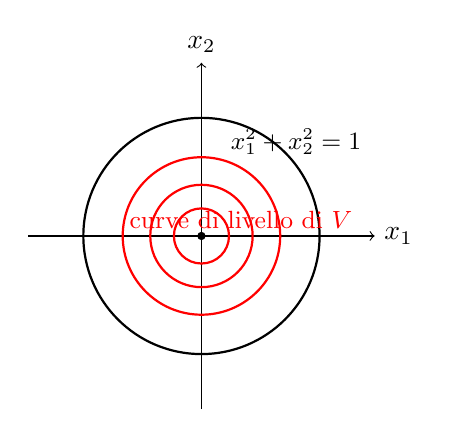
\begin{tikzpicture}[scale=1.0]
    \draw[->] (-2.2,0) -- (2.2,0) node[right] {$x_1$};
    \draw[->] (0,-2.2) -- (0,2.2) node[above] {$x_2$};

    \draw[thick] (0,0) circle (1.5);
    \node at (1.2,1.2) {\small \(x_1^2+x_2^2=1\)};

    \draw[red,thick] (0,0) circle (0.35);
    \draw[red,thick] (0,0) circle (0.65);
    \draw[red,thick] (0,0) circle (1.0);
    \fill (0,0) circle (1.5pt);

    \node[red] at (0.5,0.2) {\small curve di livello di \(V\)};
\end{tikzpicture}
\caption{Per il sistema \eqref{eq:L22-sistema-rotazione}, all'interno del disco unitario \(L_fV<0\): le curve di livello di \(V\) forniscono una stima della regione di attrazione.}
\end{figure}

\subsection{Osservazione importante}

In questo esempio il teorema di Lyapunov fornisce una \emph{stima} della regione di attrazione.  
Non sempre la stima coincide con la regione di attrazione esatta.

In realtà, per questo sistema si può andare oltre introducendo coordinate polari:
\[
x_1=r\cos\theta,
\qquad
x_2=r\sin\theta.
\]
Si ottiene
\[
\dot r = r(r^2-1),
\qquad
\dot\theta = 1.
\]
Da qui si vede subito che:
\begin{itemize}
    \item se \(0<r<1\), allora \(\dot r<0\), quindi \(r(t)\to 0\);
    \item se \(r>1\), allora \(\dot r>0\), quindi il raggio cresce.
\end{itemize}
Quindi in questo caso
\[
\mathcal{R}_{AS}(0)=B_1.
\]
Il metodo di Lyapunov aveva già individuato correttamente tale regione.

\section{Come si stima la regione di attrazione}

L'esempio precedente suggerisce un principio generale molto utile.

Supponiamo di avere:
\begin{itemize}
    \item una funzione \(V\) positiva definita;
    \item un insieme definito da una curva di livello
    \[
    C_c=\{x:V(x)=c\};
    \]
    \item la proprietà
    \[
    L_fV(x)<0
    \quad \text{all'interno di } C_c.
    \]
\end{itemize}

Allora l'insieme
\[
\Omega_c=\{x:V(x)\le c\}
\]
è positivamente invariante e, se contiene l'origine ed è contenuto in una zona in cui valgono le ipotesi del teorema, fornisce una stima della regione di attrazione.

\medskip

\noindent
In pratica si procede così:
\begin{enumerate}
    \item si sceglie una funzione \(V\) semplice;
    \item si calcola \(L_fV\);
    \item si individua una curva di livello di \(V\) all'interno della quale \(L_fV<0\);
    \item l'interno di quella curva è una stima della RAS.
\end{enumerate}

\section{Condizione di globalità: crescita radiale di \(V\)}

Per ottenere \textbf{stabilità asintotica globale} non basta che \(V\) sia positiva definita e che \(L_fV<0\).  
Occorre anche che le curve di livello di \(V\) chiudano tutto lo spazio, cioè che \(V\) cresca indefinitamente quando \(\|x\|\to\infty\).

\medskip

\noindent
\textbf{Condizione tipica di globalità.}
Se:
\begin{itemize}
    \item \(V\) è positiva definita in tutto \(\mathbb{R}^n\),
    \item \(L_fV\) è negativa definita in tutto \(\mathbb{R}^n\),
    \item
    \[
    \lim_{\|x\|\to\infty} V(x)=+\infty,
    \]
\end{itemize}
allora l'origine è \textbf{globalmente asintoticamente stabile}.

L'ultima condizione si chiama spesso \textbf{radialmente illimitata} o \textbf{proper}.

\subsection{Esempio di funzione non radialmente illimitata}

Consideriamo
\[
V(x_1,x_2)=\frac{x_1^2}{1+x_1^2}+x_2^2.
\]
Si ha:
\[
V(0,0)=0,
\qquad
V(x_1,x_2)>0 \ \text{per } (x_1,x_2)\neq (0,0),
\]
quindi \(V\) è positiva definita.

Però non è radialmente illimitata. Infatti, lungo l'asse \(x_2=0\),
\[
V(x_1,0)=\frac{x_1^2}{1+x_1^2}\xrightarrow[|x_1|\to\infty]{}1.
\]
Quindi
\[
\lim_{\|x\|\to\infty}V(x)\neq +\infty.
\]

Questo significa che le curve di livello possono non chiudersi a infinito e quindi \(V\) non è adatta, da sola, a concludere la stabilità globale.

\begin{figure}[h!]
\centering
\begin{tikzpicture}[scale=0.95]
    \draw[->] (-3.5,0) -- (3.5,0) node[right] {$x_1$};
    \draw[->] (0,-3.0) -- (0,3.0) node[above] {$x_2$};

    \draw[blue,thick]
        plot[smooth cycle,tension=0.9]
        coordinates {(0,1.3) (0.8,1.05) (1.6,0.55) (2.8,0.2) (1.6,-0.55) (0.8,-1.05) (0,-1.3) (-0.8,-1.05) (-1.6,-0.55) (-2.8,0.2) (-1.6,0.55) (-0.8,1.05)};
    \draw[dashed,blue]
        plot[smooth cycle,tension=0.9]
        coordinates {(0,2.0) (1.0,1.55) (2.2,1.0) (3.2,0.55) (2.2,-1.0) (1.0,-1.55) (0,-2.0) (-1.0,-1.55) (-2.2,-1.0) (-3.2,0.55) (-2.2,1.0) (-1.0,1.55)};
\end{tikzpicture}
\caption{Schema qualitativo di curve di livello di una funzione positiva definita ma non radialmente illimitata.}
\end{figure}

\section{Esempio parametrico e limiti del metodo indiretto}

Consideriamo il sistema
\begin{equation}
\label{eq:L22-esempio-parametrico}
\begin{cases}
\dot x_1 = -x_1-(x_2-1)^2,\\[4pt]
\dot x_2 = k(x_2-1)+4x_1(x_2-1),
\end{cases}
\qquad k\in\mathbb{R}.
\end{equation}

\subsection{Traslazione delle coordinate}

Poiché compare naturalmente il termine \(x_2-1\), è comodo traslare il sistema ponendo
\[
z_1=x_1,
\qquad
z_2=x_2-1.
\]
Allora il sistema diventa
\begin{equation}
\label{eq:L22-z}
\begin{cases}
\dot z_1 = -z_1-z_2^2,\\[4pt]
\dot z_2 = kz_2+4z_1z_2.
\end{cases}
\end{equation}

\subsection{Equilibri}

Gli equilibri soddisfano
\[
\begin{cases}
0=-z_1-z_2^2,\\
0=z_2(k+4z_1).
\end{cases}
\]
Dalla seconda equazione distinguiamo due casi.

\paragraph{Caso 1: \(z_2=0\).}
Allora la prima equazione dà
\[
z_1=0.
\]
Quindi esiste sempre l'equilibrio
\[
(0,0).
\]

\paragraph{Caso 2: \(z_2\neq 0\).}
Allora deve valere
\[
k+4z_1=0
\quad \Longrightarrow \quad
z_1=-\frac{k}{4}.
\]
Sostituendo nella prima:
\[
0=-\left(-\frac{k}{4}\right)-z_2^2
=
\frac{k}{4}-z_2^2,
\]
cioè
\[
z_2^2=\frac{k}{4}.
\]
Questa equazione ammette soluzioni reali se e solo se \(k\ge 0\). In tal caso:
\[
z_2=\pm \frac{\sqrt{k}}{2}.
\]
Quindi, per \(k\ge 0\), compaiono anche due ulteriori equilibri:
\[
\left(-\frac{k}{4},\frac{\sqrt{k}}{2}\right),
\qquad
\left(-\frac{k}{4},-\frac{\sqrt{k}}{2}\right).
\]

Tornando alle coordinate originali:
\[
x_1=z_1,
\qquad
x_2=z_2+1,
\]
gli equilibri sono:
\[
(0,1)
\]
per ogni \(k\), e inoltre, se \(k\ge 0\),
\[
\left(-\frac{k}{4},\,1+\frac{\sqrt{k}}{2}\right),
\qquad
\left(-\frac{k}{4},\,1-\frac{\sqrt{k}}{2}\right).
\]

\subsection{Stabilità dell'equilibrio \((0,0)\) in coordinate \(z\)}

Il Jacobiano del sistema \eqref{eq:L22-z} è
\[
A(z)=
\begin{pmatrix}
-1 & -2z_2\\
4z_2 & k+4z_1
\end{pmatrix}.
\]
Valutando nell'origine:
\[
A(0,0)=
\begin{pmatrix}
-1 & 0\\
0 & k
\end{pmatrix}.
\]
Gli autovalori sono quindi
\[
\lambda_1=-1,
\qquad
\lambda_2=k.
\]

Da qui segue subito:
\begin{itemize}
    \item se \(k<0\), allora entrambi gli autovalori hanno parte reale negativa, quindi l'origine è \textbf{asintoticamente stabile};
    \item se \(k>0\), allora c'è un autovalore positivo, quindi l'origine è \textbf{instabile};
    \item se \(k=0\), il metodo indiretto è \textbf{inconcludente}.
\end{itemize}

\subsection{Caso critico \(k=0\): uso di Lyapunov}

Per \(k=0\) il sistema diventa
\[
\begin{cases}
\dot z_1 = -z_1-z_2^2,\\[4pt]
\dot z_2 = 4z_1z_2.
\end{cases}
\]
Il linearizzato in \((0,0)\) è
\[
A_0=
\begin{pmatrix}
-1 & 0\\
0 & 0
\end{pmatrix},
\]
quindi il metodo indiretto non basta.

Scegliamo la funzione
\[
V(z_1,z_2)=\frac{1}{2}\bigl(4z_1^2+z_2^2\bigr).
\]
Essa è positiva definita. La derivata lungo le traiettorie è
\[
L_fV = 4z_1\dot z_1 + z_2\dot z_2.
\]
Sostituendo:
\begin{align*}
L_fV
&=
4z_1(-z_1-z_2^2)+z_2(4z_1z_2)\\
&=
-4z_1^2-4z_1z_2^2+4z_1z_2^2\\
&=
-4z_1^2\le 0.
\end{align*}
Quindi \(L_fV\) è negativa semidefinita.

Con il solo teorema diretto classico concludiamo subito che l'origine è \textbf{stabile}.  
Per concludere l'asintotica stabilità, però, serve un passo in più.

\section{Richiamo al principio di invarianza di LaSalle}

Quando \(L_fV\le 0\) ma non è negativa definita, il teorema diretto di Lyapunov garantisce la stabilità, ma non sempre l'asintotica stabilità. In questi casi si guarda il sottoinsieme
\[
E=\{x : L_fV(x)=0\}.
\]

Nel caso in esame,
\[
L_fV(z_1,z_2)=-4z_1^2,
\]
quindi
\[
E=\{(z_1,z_2): z_1=0\}.
\]
Studiamo la dinamica su \(E\). Se \(z_1=0\), il sistema diventa
\[
\begin{cases}
\dot z_1=-z_2^2,\\
\dot z_2=0.
\end{cases}
\]
Affinché una traiettoria resti per sempre in \(E\), deve valere anche \(\dot z_1=0\), cioè
\[
-z_2^2=0 \quad \Longrightarrow \quad z_2=0.
\]
Dunque l'unico insieme invariante contenuto in \(E\) è il solo punto
\[
(0,0).
\]

Per il principio di LaSalle si conclude che, per \(k=0\), l'origine è \textbf{asintoticamente stabile}.

\medskip

\noindent
Riassumendo per l'equilibrio \((0,0)\) del sistema \eqref{eq:L22-z}:
\[
\boxed{
\begin{array}{ll}
k<0 & \Rightarrow \text{origine asintoticamente stabile},\\[4pt]
k=0 & \Rightarrow \text{origine asintoticamente stabile (via Lyapunov + LaSalle)},\\[4pt]
k>0 & \Rightarrow \text{origine instabile}.
\end{array}
}
\]

\section{Osservazione sul ritratto di fase nel caso \(k=0\)}

Nel caso \(k=0\), il sistema
\[
\begin{cases}
\dot z_1=-z_1-z_2^2,\\
\dot z_2=4z_1z_2
\end{cases}
\]
mostra bene perché la sola semidefinità negativa di \(L_fV\) non impedisce comunque la convergenza all'origine.

Infatti:
\begin{itemize}
    \item se \(z_1>0\), il termine \(-z_1\) tende a spingere \(z_1\) verso sinistra;
    \item il termine \(-z_2^2\) rende \(\dot z_1\) ancora più negativo;
    \item la dinamica di \(z_2\) dipende dal prodotto \(z_1z_2\), quindi cambia segno a seconda dei quadranti.
\end{itemize}

Le traiettorie vengono comunque progressivamente riportate verso l'origine.  
Il ritratto di fase suggerisce la stessa conclusione ottenuta rigorosamente con LaSalle.

\begin{figure}[h!]
\centering
\begin{tikzpicture}[scale=1.0]
    \draw[->] (-3.2,0) -- (3.2,0) node[right] {$z_1$};
    \draw[->] (0,-3.0) -- (0,3.0) node[above] {$z_2$};

    % nullcline z1 = -z2^2
    \draw[orange,thick,domain=-1.6:1.6,samples=100]
        plot ({-(\x*\x)}, {\x});
    \node[orange] at (-2.2,2.2) {\small \(z_1=-z_2^2\)};

    % z2=0
    \draw[blue,thick] (-3,0) -- (3,0);
    \node[blue] at (2.3,0.25) {\small \(z_2=0\)};

    \fill (0,0) circle (1.8pt);

    % qualitative arrows
    \draw[-{Latex[length=2.5mm]},red] (1.8,2.0) -- (1.25,1.8);
    \draw[-{Latex[length=2.5mm]},red] (1.8,-2.0) -- (1.25,-1.8);
    \draw[-{Latex[length=2.5mm]},red] (-2.0,2.0) -- (-2.2,1.4);
    \draw[-{Latex[length=2.5mm]},red] (-2.0,-2.0) -- (-2.2,-1.4);
    \draw[-{Latex[length=2.5mm]},red] (0.9,0.7) -- (0.25,0.45);
    \draw[-{Latex[length=2.5mm]},red] (0.9,-0.7) -- (0.25,-0.45);
\end{tikzpicture}
\caption{Schema qualitativo del ritratto di fase per il caso \(k=0\).}
\end{figure}

\section{Conclusioni operative della lezione}

Questa lezione chiarisce alcuni punti molto importanti.

\subsection*{1. Il metodo diretto può riuscire quando il linearizzato fallisce}
Negli esempi
\[
\dot x=-x^3
\qquad \text{e} \qquad
\dot x=x^3
\]
il linearizzato nell'origine è nullo e quindi non conclude nulla; il metodo diretto di Lyapunov invece distingue perfettamente il caso stabile da quello instabile.

\subsection*{2. Le curve di livello di \(V\) servono anche a stimare la RAS}
Non servono solo a dimostrare la stabilità locale, ma anche a costruire insiemi invarianti contenuti nella regione di attrazione.

\subsection*{3. Per la stabilità globale serve una condizione di crescita a infinito}
La proprietà
\[
\lim_{\|x\|\to\infty}V(x)=+\infty
\]
è fondamentale se si vuole passare da una conclusione locale a una conclusione globale.

\subsection*{4. Se \(L_fV\) è solo semidefinita, spesso bisogna usare LaSalle}
Il teorema diretto classico dà la stabilità.  
Per l'asintotica stabilità bisogna studiare l'insieme
\[
\{x : L_fV(x)=0\}
\]
e cercare il suo massimo insieme invariante.

\section{Schema riassuntivo}

Per un sistema autonomo con equilibrio nell'origine:
\[
\dot x=f(x),
\qquad
f(0)=0,
\]
si cerca una funzione \(V\) tale che:
\begin{itemize}
    \item \(V(x)>0\) per \(x\neq 0\);
    \item \(V(0)=0\);
    \item \(L_fV(x)\le 0\) oppure \(<0\).
\end{itemize}

Allora:
\[
\boxed{
\begin{array}{ll}
V \text{ p.d.},\ L_fV\le 0
&\Rightarrow \text{origine stabile},\\[4pt]
V \text{ p.d.},\ L_fV<0
&\Rightarrow \text{origine asintoticamente stabile},\\[4pt]
V \text{ p.d.},\ L_fV>0
&\Rightarrow \text{origine instabile}.
\end{array}
}
\]

Se inoltre
\[
\lim_{\|x\|\to\infty}V(x)=+\infty,
\]
si può spesso concludere la \textbf{stabilità asintotica globale}.

\medskip

\noindent
Questa è l'idea di fondo che useremo anche nelle lezioni successive: costruire una funzione scalare semplice che catturi il comportamento qualitativo di un sistema non lineare, anche quando risolverlo esplicitamente è impossibile.